%!TEX root = ../slides.tex

\section[eDSL for the SDR]{Embedded Domain Specific Language for the Software-defined Radio}

\subsection[Existing Solutions]{Existing Solutions}

\begin{frame}{Existing Solutions}
  \vfill
  \begin{itemize}
    \item Dedicated languages based on the dataflow model~\cite{Dennis1980,Engels1994}
    \item GNU Radio~\cite{GNURadio}
  \end{itemize}
  \vfill
\end{frame}

\subsection[Proposed eDSL]{Description of the Proposed Embedded Domain Specific Language}

\begin{frame}{Proposed eDSL}
  \vfill
  \begin{itemize}
    \item Concepts:
    \begin{itemize}
      \item Close to cyclo-static dataflow model but not stateless
      \item Domain specific language embedded in \Cxx
      \item Compilation is performed at runtime, meta-programming technique is avoided
    \end{itemize}
    \vspace{0.3cm}
    \item Objectives:
    \begin{itemize}
      \item High performance eDSL
      \item Integrate the eDSL with \AFFECT and its fast implementations
      \item Easy to understand, to use and to modify for new users
    \end{itemize}
  \end{itemize}
  \vfill
\end{frame}

\begin{frame}{Tasks and Sequence}
  \vfill
  \begin{columns}
    \begin{column}[T]{6cm}
    \begin{figure}[!h]
      \centering
      \scalebox{.65}{
      \begin{tikzpicture}%[scale=\tikzscale]
          \tikzset{ tsk/.style ={draw=Paired-1, rounded corners=0pt, text=Paired-1, minimum height=1.0cm, minimum width=1cm} }
          \tikzset{ ss/.style  ={draw=Paired-9, rounded corners=2pt, minimum height=1.5cm} }
          \tikzset{ seq/.style ={draw=Paired-11, rounded corners=2pt} }
          \tikzset{ sin/.style ={draw=Paired-7, circle, minimum width=0.3cm, text=black, preaction={fill=white}, pattern=north east lines, pattern color=Paired-7} }
          \tikzset{ sout/.style={draw=Paired-5, circle, minimum width=0.3cm, text=black, preaction={fill=white}, pattern=crosshatch dots, pattern color=Paired-5} }

          \draw[->,>=latex,dotted,white] (-1.25,0) -- (-0.5,0.0) node [midway, above] {};
          \draw[->,>=latex,dotted,white] (6.5,0) -- (6+1.25,0) node [midway, above] {};

          \node[tsk ] (t1) at (0.0, 0.00) {$t_1$};
          \node[sout] (t1_so) at (0.0+0.5, 0) {};
          \node[tsk ] (t2) at (2.0, 0.00) {$t_2$};
          \node[sin ] (t2_si) at (2.0-0.5, 0) {};
          \node[sout] (t2_so) at (2.0+0.5, 0) {};
          \node[tsk ] (t3) at (4.0, 0.00) {$t_3$};
          \node[sin ] (t3_si) at (4.0-0.5, 0) {};
          \node[sout] (t3_so) at (4.0+0.5, 0) {};
          \node[tsk ] (t4) at (6.0, 0.00) {$t_4$};
          \node[sin ] (t4_si) at (6.0-0.5, 0) {};

          \draw[->,>=latex] (t1_so) -- (t2_si) node [midway, above] {};
          \draw[->,>=latex] (t2_so) -- (t3_si) node [midway, above] {};
          \draw[->,>=latex] (t3_so) -- (t4_si) node [midway, above] {};

          \node[seq, label={[Paired-11]below:Sequence},  dashed, fit=(t1) (t4)] {};

          \node[draw=Paired-1, rounded corners=0pt,         minimum height=0.3cm, minimum width=0.7cm, text=Paired-1, label={[Paired-1]right:Task}         ] (l1) at (+0.0, 1.9) {};
      %   \node[draw=Paired-3, rounded corners=2pt, dashed, minimum height=0.3cm, minimum width=0.7cm, text=Paired-1, label={[Paired-3]right:Module}       ] (l2) at (+0.0, 1.9) {};
          \node[sout,                                                                                                 label={[Paired-5]right:Output socket}] (l3) at (+4.0, 1.3) {};
          \node[sin,                                                                                                  label={[Paired-7]right:Input socket} ] (l4) at (+4.0, 1.9) {};
      \end{tikzpicture}
      }
    \end{figure}
    \end{column}
    \begin{column}[T]{6cm}
    \begin{figure}[!h]
      \centering
      \scalebox{.65}{
      \begin{tikzpicture}%[scale=\tikzscale]
        \tikzset{ tsk/.style ={draw=Paired-1, rounded corners=0pt, text=Paired-1, minimum height=1.0cm, minimum width=1cm} }
        \tikzset{ ss/.style  ={draw=Paired-9, rounded corners=2pt, minimum height=1.5cm} }
        \tikzset{ seq/.style ={draw=Paired-11, rounded corners=2pt, minimum height=1.5cm} }
        \tikzset{ sin/.style ={draw=Paired-7, circle, minimum width=0.3cm, text=black, preaction={fill=white}, pattern=north east lines, pattern color=Paired-7} }
        \tikzset{ sout/.style={draw=Paired-5, circle, minimum width=0.3cm, text=black, preaction={fill=white}, pattern=crosshatch dots, pattern color=Paired-5} }

        \node[tsk ] (t1)    at (0.0    , +1.00) {$t_1$};
        \node[sin ] (t1_si) at (0.0-0.5, +1.00) {};
        \node[sout] (t1_so) at (0.0+0.5, +1.00) {};

        \node[tsk ] (t2)     at (2.0    ,  0.00) {$t_2$};
        \node[sin ] (t2_si) at (2.0-0.5,  0.00) {};
        \node[sout] (t2_so) at (2.0+0.5,  0.00) {};

        \node[tsk ] (t3)    at (0.0    , -1.00) {$t_3$};
        \node[sin ] (t3_si) at (0.0-0.5, -1.00) {};
        \node[sout] (t3_so) at (0.0+0.5, -1.00) {};

        \node[tsk ] (t4)     at (4.0    ,  0.00) {$t_4$};
        \node[sin ] (t4_si1) at (4.0-0.5,  0.25) {};
        \node[sin ] (t4_si2) at (4.0-0.5, -0.25) {};
        \node[sout] (t4_so)  at (4.0+0.5,  0.00) {};

        \node[tsk ] (t5)    at (6.0,     +1.00) {$t_5$};
        \node[sin ] (t5_si) at (6.0-0.5, +1.00) {};
        \node[sout] (t5_so) at (6.0+0.5, +1.00) {};

        \node[tsk ] (t6)    at (6.0,     -1.00) {$t_6$};
        \node[sin ] (t6_si) at (6.0-0.5, -1.00) {};
        \node[sout] (t6_so) at (6.0+0.5, -1.00) {};

        \draw[->,>=latex] (t1_so) -- (t2_si)  node [midway, above] {};
        \draw[->,>=latex] (t2_so) -- (t4_si1) node [midway, above] {};
        \draw[->,>=latex] (t3_so) -- (3,-1) |- (t4_si2) node [midway, above] {};
        \draw[->,>=latex] (t4_so) -- (t5_si)  node [midway, above] {};
        \draw[->,>=latex] (t4_so) -- (t6_si)  node [midway, above] {};

        \draw[->,>=latex,dotted] (-1.25,+1) -- (t1_si) node [midway, above] {};
        \draw[->,>=latex,dotted] (-1.25,-1) -- (t3_si) node [midway, above] {};

        \draw[->,>=latex,dotted] (t5_so) -- (6+1.25,+1) node [midway, above] {};
        \draw[->,>=latex,dotted] (t6_so) -- (6+1.25,-1) node [midway, above] {};

        \node[seq, label={[Paired-11]below:Sequence},  dashed, fit=(t1_si) (t1) (t2) (t3) (t5_so)] {};
      \end{tikzpicture}
      }
    \end{figure}
    \end{column}
  \end{columns}
  \vfill
  \begin{itemize}
    \item A sequence is build from an initial and a final list of tasks
    \item The tasks scheduling order inside a sequence is determined at the construction
    \begin{itemize}
      \item Could be resolved at compilation time
      \item But small overhead at runtime
    \end{itemize}
    \item Binding rules
    \begin{itemize}
      \item All the input sockets of a task have to be bound to execute a task
      \item An input socket has to be bound to a single output socket
      \item An output socket can be bound to many input sockets
    \end{itemize}
  \end{itemize}
  \vfill
\end{frame}

\begin{frame}{Parallelization Techniques}
  \begin{columns}
    \begin{column}[T]{6cm}
    \underline{Sequence duplication:}

    \vspace{0.2cm}
    \begin{figure}[!h]
      \centering
      \scalebox{.45}{
      \begin{tikzpicture}%[scale=\tikzscale]
        \tikzset{ tsk/.style ={draw=Paired-1, rounded corners=0pt, text=Paired-1, minimum height=1.0cm, minimum width=1cm} }
        \tikzset{ ss/.style  ={draw=Paired-9, rounded corners=2pt, minimum height=1.5cm} }
        \tikzset{ seq/.style ={draw=Paired-11, rounded corners=2pt} }
        \tikzset{ sin/.style ={draw=Paired-7, circle, minimum width=0.3cm, text=black, preaction={fill=white}, pattern=north east lines, pattern color=Paired-7} }
        \tikzset{ sout/.style={draw=Paired-5, circle, minimum width=0.3cm, text=black, preaction={fill=white}, pattern=crosshatch dots, pattern color=Paired-5} }

        \draw[->,>=latex,dotted,white] (-1.25,0) -- (-0.5,0.0) node [midway, above] {};
        \draw[->,>=latex,dotted,white] (6.5,0) -- (6+1.25,0) node [midway, above] {};

        \newcommand\thr{0}

        \thread{(-1,\thr-0.5)}{1}{th1};
        \node[tsk ] (t1)    at (0.0    , \thr) {$t_1^1$};
        \node[sout] (t1_so) at (0.0+0.5, \thr) {};
        \node[tsk ] (t2)    at (2.0    , \thr) {$t_2^1$};
        \node[sin ] (t2_si) at (2.0-0.5, \thr) {};
        \node[sout] (t2_so) at (2.0+0.5, \thr) {};
        \node[tsk ] (t3)    at (4.0    , \thr) {$t_3^1$};
        \node[sin ] (t3_si) at (4.0-0.5, \thr) {};
        \node[sout] (t3_so) at (4.0+0.5, \thr) {};
        \node[tsk ] (t4)    at (6.0    , \thr) {$t_4^1$};
        \node[sin ] (t4_si) at (6.0-0.5, \thr) {};

        \draw[->,>=latex] (t1_so) -- (t2_si) node [midway, above] {};
        \draw[->,>=latex] (t2_so) -- (t3_si) node [midway, above] {};
        \draw[->,>=latex] (t3_so) -- (t4_si) node [midway, above] {};

        \newcommand\tthr{-1.5}

        \thread{(-1,-2)}{1}{th2};
        \node[tsk ] (tt1)    at (0.0    , \tthr) {$t_1^2$};
        \node[sout] (tt1_so) at (0.0+0.5, \tthr) {};
        \node[tsk ] (tt2)    at (2.0    , \tthr) {$t_2^2$};
        \node[sin ] (tt2_si) at (2.0-0.5, \tthr) {};
        \node[sout] (tt2_so) at (2.0+0.5, \tthr) {};
        \node[tsk ] (tt3)    at (4.0    , \tthr) {$t_3^2$};
        \node[sin ] (tt3_si) at (4.0-0.5, \tthr) {};
        \node[sout] (tt3_so) at (4.0+0.5, \tthr) {};
        \node[tsk ] (tt4)    at (6.0    , \tthr) {$t_4^2$};
        \node[sin ] (tt4_si) at (6.0-0.5, \tthr) {};

        \draw[->,>=latex] (tt1_so) -- (tt2_si) node [midway, above] {};
        \draw[->,>=latex] (tt2_so) -- (tt3_si) node [midway, above] {};
        \draw[->,>=latex] (tt3_so) -- (tt4_si) node [midway, above] {};

        \newcommand\tttthr{-3.5}

        \thread{(-1,-4)}{1}{tht};
        \node[tsk ] (tttt1)    at (0.0    , \tttthr) {$t_1^t$};
        \node[sout] (tttt1_so) at (0.0+0.5, \tttthr) {};
        \node[tsk ] (tttt2)    at (2.0    , \tttthr) {$t_2^t$};
        \node[sin ] (tttt2_si) at (2.0-0.5, \tttthr) {};
        \node[sout] (tttt2_so) at (2.0+0.5, \tttthr) {};
        \node[tsk ] (tttt3)    at (4.0    , \tttthr) {$t_3^t$};
        \node[sin ] (tttt3_si) at (4.0-0.5, \tttthr) {};
        \node[sout] (tttt3_so) at (4.0+0.5, \tttthr) {};
        \node[tsk ] (tttt4)    at (6.0    , \tttthr) {$t_4^t$};
        \node[sin ] (tttt4_si) at (6.0-0.5, \tttthr) {};

        \draw[->,>=latex] (tttt1_so) -- (tttt2_si) node [midway, above] {};
        \draw[->,>=latex] (tttt2_so) -- (tttt3_si) node [midway, above] {};
        \draw[->,>=latex] (tttt3_so) -- (tttt4_si) node [midway, above] {};

        \draw[-,>=latex,dotted] (tt1) -- (tttt1) node [midway, above] {};
        \draw[-,>=latex,dotted] (tt2) -- (tttt2) node [midway, above] {};
        \draw[-,>=latex,dotted] (tt3) -- (tttt3) node [midway, above] {};
        \draw[-,>=latex,dotted] (tt4) -- (tttt4) node [midway, above] {};

        \node[seq, label={[Paired-11]below:Sequence},  dashed, fit=(t1) (tttt1) (t4) (th1)] {};
      \end{tikzpicture}
      }
    \end{figure}
    \end{column}
    \begin{column}[T]{6cm}
    \underline{Sequence pipelining:}

    \vspace{0.2cm}
    \begin{figure}[!h]
      \centering
      \scalebox{.45}{
      \begin{tikzpicture}%[scale=\tikzscale]
        \tikzset{ tsk/.style ={draw=Paired-1, rounded corners=0pt, text=Paired-1, minimum height=1.0cm, minimum width=1cm} }
        \tikzset{ stsk/.style ={draw=Paired-1, rounded corners=0pt, text=Paired-1, minimum height=1.0cm, minimum width=1cm, fill=Paired-1!7} }
        \tikzset{ ss/.style  ={draw=Paired-9, rounded corners=2pt, minimum height=1.5cm} }
        \tikzset{ seq/.style ={draw=Paired-11,  dashed, rounded corners=2pt} }
        % \tikzset{ pip/.style ={draw=Dark2-1,  dashed, rounded corners=2pt} }
        \tikzset{ pip/.style ={draw=Dark2-8,  dotted, thick, rounded corners=2pt} }
        \tikzset{ sin/.style ={draw=Paired-7, circle, minimum width=0.3cm, text=black, preaction={fill=white}, pattern=north east lines, pattern color=Paired-7} }
        \tikzset{ sout/.style={draw=Paired-5, circle, minimum width=0.3cm, text=black, preaction={fill=white}, pattern=crosshatch dots, pattern color=Paired-5} }

        \newcommand\thr{0}

        \node[stsk] (t1)    at ( 0.0    , \thr) {$t_1$};
        \node[sout] (t1_so) at ( 0.0+0.5, \thr) {};
        \node[tsk ] (t2)    at ( 2.0    , \thr) {$t_2$};
        \node[sin ] (t2_si) at ( 2.0-0.5, \thr) {};
        \node[sout] (t2_so) at ( 2.0+0.5, \thr) {};
        \node[tsk ] (t3)    at ( 4.0    , \thr) {$t_3$};
        \node[sin ] (t3_si) at ( 4.0-0.5, \thr) {};
        \node[sout] (t3_so) at ( 4.0+0.5, \thr) {};
        \node[tsk ] (t4)    at ( 6.0    , \thr) {$t_4$};
        \node[sin ] (t4_si) at ( 6.0-0.5, \thr) {};
        \node[sout] (t4_so) at ( 6.0+0.5, \thr) {};
        \node[stsk] (t5)    at ( 8.0    , \thr) {$t_5$};
        \node[sin ] (t5_si) at ( 8.0-0.5, \thr) {};
        \node[sout] (t5_so) at ( 8.0+0.5, \thr) {};
        \node[stsk] (t6)    at (10.0    , \thr) {$t_6$};
        \node[sin ] (t6_si) at (10.0-0.5, \thr) {};

        \draw[->,>=latex] (t1_so) -- (t2_si) node [midway, above] {};
        \draw[->,>=latex] (t2_so) -- (t3_si) node [midway, above] {};
        \draw[->,>=latex] (t3_so) -- (t4_si) node [midway, above] {};
        \draw[->,>=latex] (t4_so) -- (t5_si) node [midway, above] {};
        \draw[->,>=latex] (t5_so) -- (t6_si) node [midway, above] {};

        \Thread{0.00}{0.7}{th1}
        \Thread{3.25}{0.7}{th2}
        \Thread{3.75}{0.7}{th3}
        \Thread{4.25}{0.7}{th4}
        \Thread{4.75}{0.7}{th5}
        \Thread{9.00}{0.7}{th6}

        \node[seq, label={[Paired-11]below:Stage 1}, fit=(t1) (t1_so)                  ] (seq1) {};
        \node[seq, label={[Paired-11]below:Stage 2}, fit=(t2_si) (t2) (t3) (t4) (t4_so)] (seq2) {};
        \node[seq, label={[Paired-11]below:Stage 3}, fit=(t5_si) (t5) (t6)             ] (seq3) {};

        \node[pip, minimum height=2.5cm, minimum width=12.0cm, label={[Dark2-8]below:Pipeline}, fit=(seq1) (seq2) (seq3)] {};

        % \thread{(2.4,+1.0)}{0.5}{thl};
        % \node at (3.2,+1.25) {thread};
      \end{tikzpicture}
      }
    \end{figure}
    \end{column}
  \end{columns}

  \vspace{0.3cm}
  \begin{columns}
    \begin{column}[T]{6cm}
      \begin{itemize}
        \item Put each duplicated sequence on a thread
        \item Preserve the cache locality if the same thread remains on the same core
      \end{itemize}
    \end{column}
    \begin{column}[T]{6cm}
      \begin{itemize}
        \item Some tasks cannot be duplicated because of sequential dependency on themselves
        \item Splitting a sequence in stages allow to parallelize the overall application
        \item Duplicating a stage remains possible if all the containing tasks are not sequential
      \end{itemize}
    \end{column}
  \end{columns}

\end{frame}

\subsection[DVB-S2 Standard]{Application on the DVB-S2 Standard}

\begin{frame}{Objectives}
  \vspace{-0.1cm}
  \begin{figure}[htp]
    \centering
    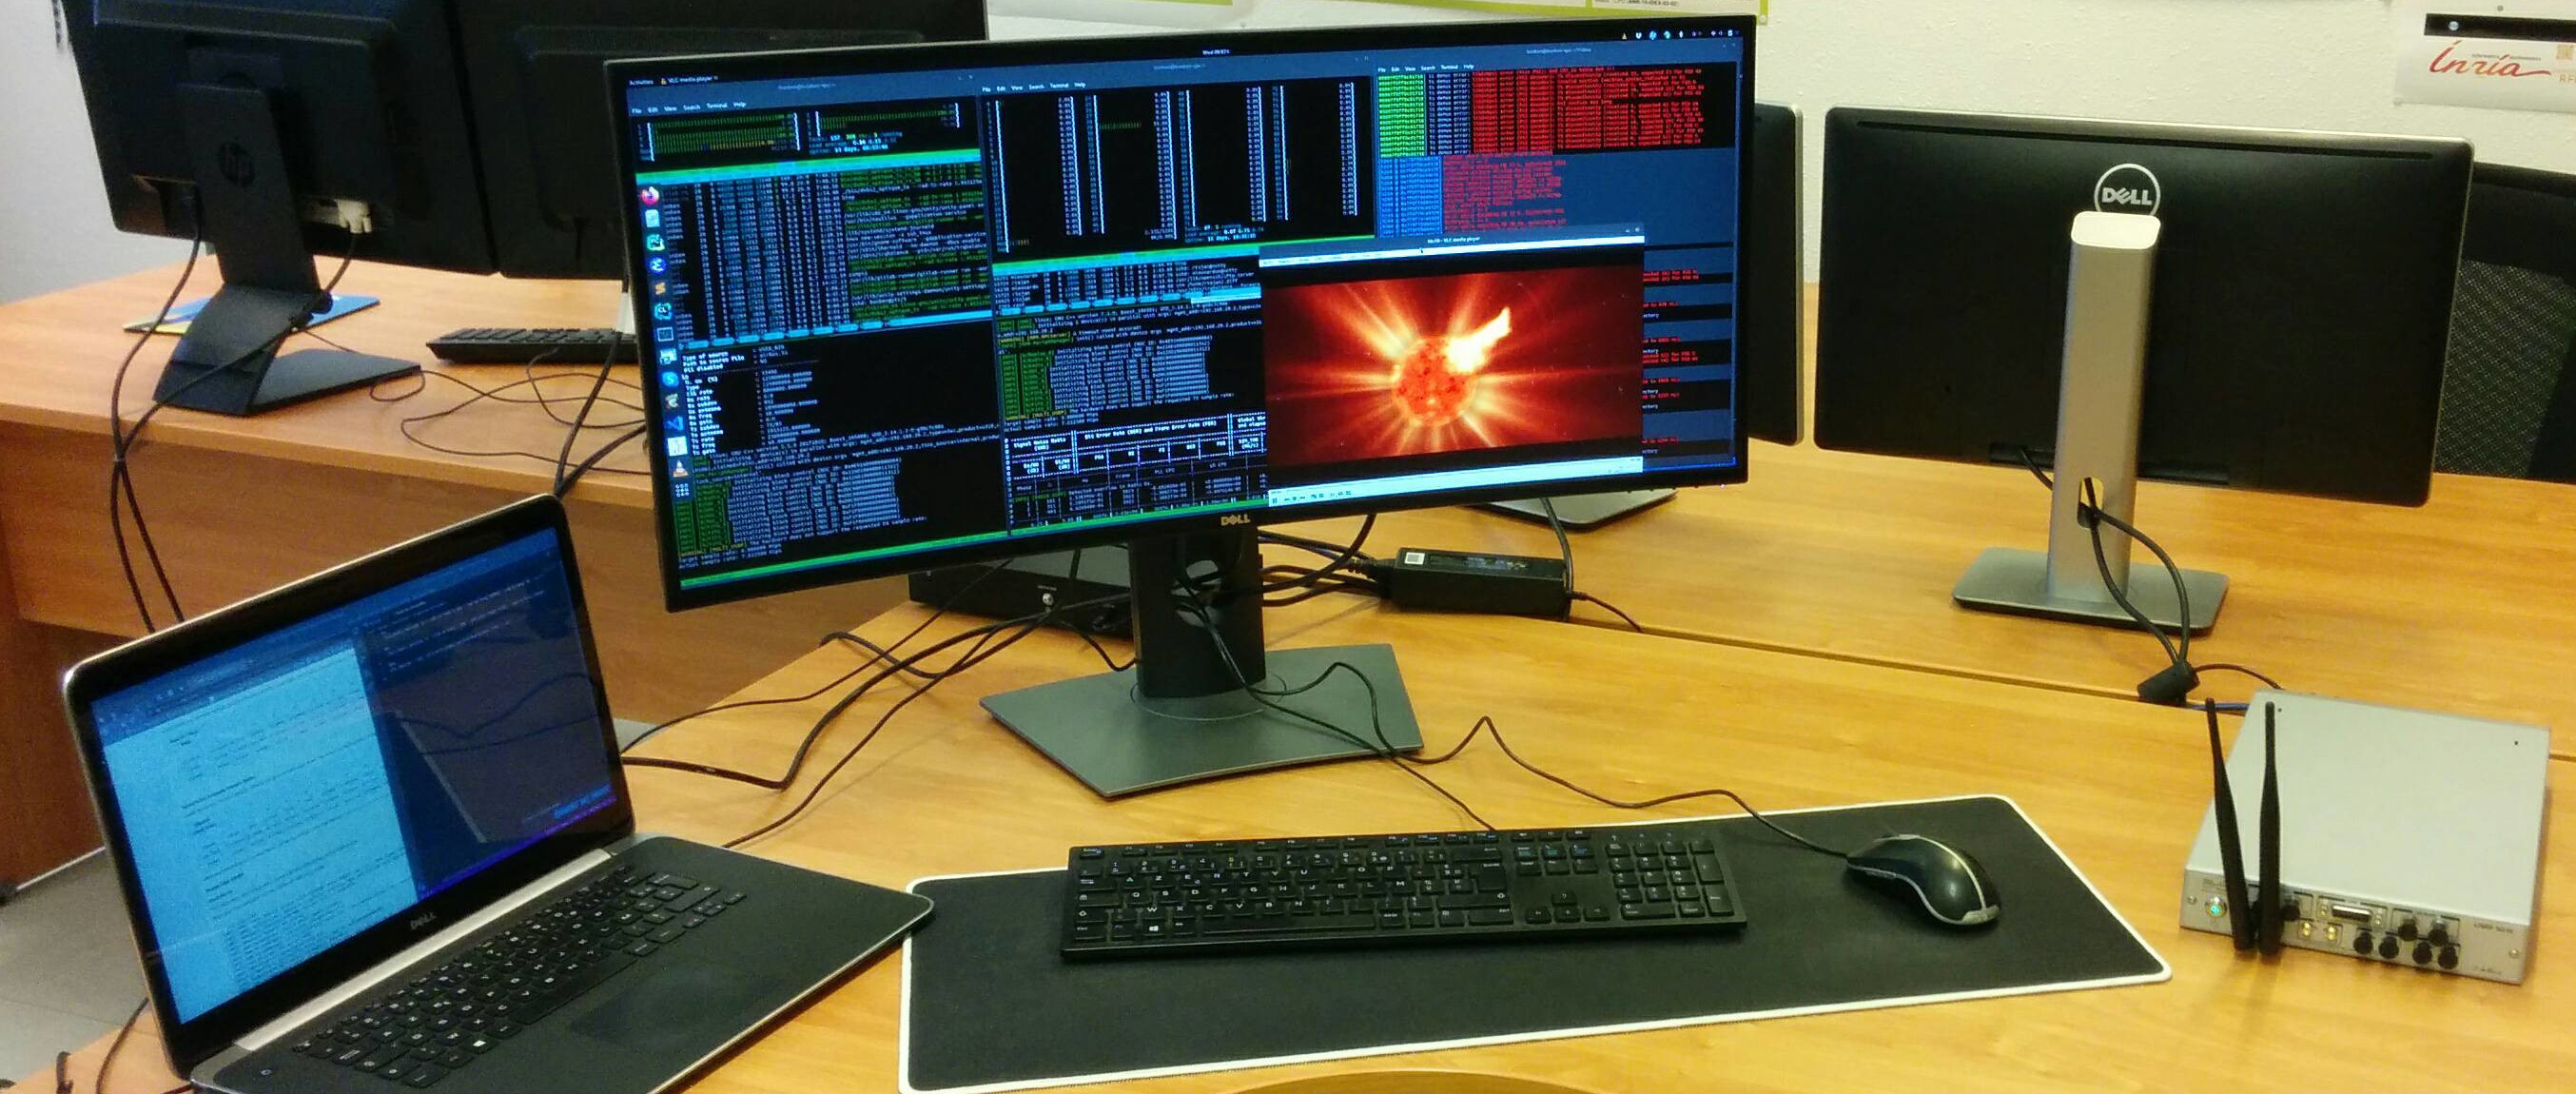
\includegraphics[scale=0.25]{pics/demo_dvbs2}
  \end{figure}
  \begin{itemize}
    \item Implement a full DVB-S2 transceiver (streaming video)
    \item Two Universal Software Radio Peripherals (USRPs) N320 for the RF
    \item One middle class computer for the transmitter (Tx) BB processing => SDR
    \item One server class computer for the receiver (Rx) BB processing => SDR
  \end{itemize}
  \vfill
  \begin{table}[htp]
    \centering
    \resizebox{1.0\linewidth}{!}{
    % \begin{tabular}{c c c c c c c c}
    %   \textbf{Config.} & \textbf{Modulation} & \textbf{Rate} $\bm{R}$ & $\bm{K_\text{\textbf{BCH}}}$ & $\bm{K_\text{\textbf{LDPC}}}$ & $\bm{N_\text{\textbf{LDPC}}}$ & $\bm{N_\text{\textbf{PLH}}}$ & \textbf{Interleaver}\\
    %   \hline \hline
    %   MODCOD 1 &  QPSK & 3/5 &  9552 &  9720 & 16200 & 16740 & no\\
    %   MODCOD 2 &  QPSK & 8/9 & 14232 & 14400 & 16200 & 16740 & no\\
    %   MODCOD 3 & 8-PSK & 8/9 & 14232 & 14400 & 16200 & 16740 & column/row\\
    % \end{tabular}
    \begin{tabular}{c c c c c c c}
      \textbf{Config.} & \textbf{Modulation} & \textbf{Rate} $\bm{R}$ & $\bm{K_\text{\textbf{BCH}}}$ & $\bm{K_\text{\textbf{LDPC}}}$ & $\bm{N_\text{\textbf{LDPC}}}$ & $\bm{\mathcal{T}_i}$ (Rx, Seq.)\\
      \hline \hline
      \textcolor{Paired-1}{MODCOD 1} &  QPSK & 3/5 &  9552 &  9720 & 16200 & 3.4 Mb/s\\
      \textcolor{Paired-3}{MODCOD 2} &  QPSK & 8/9 & 14232 & 14400 & 16200 & 4.1 Mb/s\\
      \textcolor{Paired-5}{MODCOD 3} & 8-PSK & 8/9 & 14232 & 14400 & 16200 & 4.0 Mb/s\\
    \end{tabular}
    }
    \caption*{Selected DVB-S2 configurations (MODCOD).}
  \end{table}
  \vfill

\end{frame}

\begin{frame}{Transmitter}
  \vfill
  \begin{figure}[!h]
    \centering
    \scalebox{.50}{
    \begin{tikzpicture}%[scale=\tikzscale]
      \tikzset{ tsk/.style ={draw=Paired-1, rounded corners=0pt, text=Paired-1, minimum height=1.0cm, minimum width=1cm} }
      \tikzset{ stsk/.style={draw=Paired-1, rounded corners=0pt, text=Paired-1, minimum height=1.0cm, minimum width=1cm, fill=Paired-1!7} }
      \tikzset{ ss/.style  ={draw=Paired-9, rounded corners=2pt, minimum height=1.5cm} }
      \tikzset{ seq/.style ={draw=Paired-11, dashed, rounded corners=2pt} }
      \tikzset{ mdl/.style ={draw=Paired-3,  dashed, rounded corners=2pt} }
      \tikzset{ pip/.style ={draw=Dark2-8,  dotted, thick, rounded corners=2pt} }
      \tikzset{ sin/.style ={draw=Paired-7, circle, minimum width=0.3cm, text=black, preaction={fill=white}, pattern=north east lines, pattern color=Paired-7} }
      \tikzset{ sout/.style={draw=Paired-5, circle, minimum width=0.3cm, text=black, preaction={fill=white}, pattern=crosshatch dots, pattern color=Paired-5} }

      \node[stsk                    , align=center] (t1) at (0.0, 2.0) {~generate~~\\($t^{\text{Tx}}_1$)};
      \node[tsk , right=2.00cm of t1, align=center] (t2)               {~scramble~~\\($t^{\text{Tx}}_2$)};
      \node[tsk , right=1.25cm of t2, align=center] (t3)               {~encode~~\\($t^{\text{Tx}}_3$)};
      \node[tsk , right=1.25cm of t3, align=center] (t4)               {~encode~~\\($t^{\text{Tx}}_4$)};
      \node[tsk , right=1.25cm of t4, align=center] (t5)               {~interleave~~\\($t^{\text{Tx}}_5$)};
      \node[tsk,  below=1.00cm of t2, align=center] (t6)               {~modulate~~\\($t^{\text{Tx}}_6$)};
      \node[tsk , right=1.25cm of t6, align=center] (t7)               {~insert~~\\($t^{\text{Tx}}_7$)};
      \node[tsk , right=1.25cm of t7, align=center] (t8)               {~scramble~~\\($t^{\text{Tx}}_8$)};
      \node[stsk, right=4.60cm of t8, align=center] (t9)               {~filter~~\\($t^{\text{Tx}}_9$)};
      \node[stsk, right=1.00cm of t9, align=center] (t10)              {~send~~\\($t^{\text{Tx}}_{10}$)};

      \node[sout, at=(t1.east) ] (t1_so)  {};
      \node[sin,  at=(t2.west) ] (t2_si)  {};
      \node[sout, at=(t2.east) ] (t2_so)  {};
      \node[sin,  at=(t3.west) ] (t3_si)  {};
      \node[sout, at=(t3.east) ] (t3_so)  {};
      \node[sin,  at=(t4.west) ] (t4_si)  {};
      \node[sout, at=(t4.east) ] (t4_so)  {};
      \node[sin,  at=(t5.west) ] (t5_si)  {};
      \node[sout, at=(t5.east) ] (t5_so)  {};
      \node[sin,  at=(t6.west) ] (t6_si)  {};
      \node[sout, at=(t6.east) ] (t6_so)  {};
      \node[sin,  at=(t7.west) ] (t7_si)  {};
      \node[sout, at=(t7.east) ] (t7_so)  {};
      \node[sin,  at=(t8.west) ] (t8_si)  {};
      \node[sout, at=(t8.east) ] (t8_so)  {};
      \node[sin,  at=(t9.west) ] (t9_si)  {};
      \node[sout, at=(t9.east) ] (t9_so)  {};
      \node[sin,  at=(t10.west)] (t10_si) {};

      \node[mdl, label={[Paired-3]above:Source Binary File},  fit=(t1)           (t1_so)] (m1) {};
      \node[mdl, label={[Paired-3]above:Scrambler Binary},    fit=(t2)  (t2_si)  (t2_so)] (m2) {};
      \node[mdl, label={[Paired-3]above:Encoder BCH},         fit=(t3)  (t3_si)  (t3_so)] (m3) {};
      \node[mdl, label={[Paired-3]above:Encoder LDPC},        fit=(t4)  (t4_si)  (t4_so)] (m4) {};
      \node[mdl, label={[Paired-3]above:Interleaver},         fit=(t5)  (t5_si)  (t5_so)] (m5) {};
      \node[mdl, label={[Paired-3]above:Modem PSK},           fit=(t6)  (t6_si)  (t6_so)] (m6) {};
      \node[mdl, label={[Paired-3]above:Framer PLH},          fit=(t7)  (t7_si)  (t7_so)] (m7) {};
      \node[mdl, label={[Paired-3]above:Scrambler Symbol},    fit=(t8)  (t8_si)  (t8_so)] (m8) {};
      \node[mdl, label={[Paired-3]above:Filter Shaping},      fit=(t9)  (t9_si)  (t9_so)] (m9) {};
      \node[mdl, label={[Paired-3]above:Radio},               fit=(t10) (t10_si)        ] (m9) {};

      \draw[->,>=latex] (t1_so) -- (t2_si)  node [midway, above] {};
      \draw[->,>=latex] (t2_so) -- (t3_si)  node [midway, above] {};
      \draw[->,>=latex] (t3_so) -- (t4_si)  node [midway, above] {};
      \draw[->,>=latex] (t4_so) -- (t5_si)  node [midway, above] {};
      \draw[->,>=latex] (t5_so) -- (13.9,2.0) -- (13.9,1.15) -- (2.25,1.15) -- (2.25,0) -- (t6_si)  node [midway, above] {};
      \draw[->,>=latex] (t6_so) -- (t7_si)  node [midway, above] {};
      \draw[->,>=latex] (t7_so) -- (t8_si)  node [midway, above] {};
      \draw[->,>=latex] (t8_so) -- (t9_si)  node [midway, above] {};
      \draw[->,>=latex] (t9_so) -- (t10_si) node [midway, above] {};
      \draw[black, -] (t10.east)--++(0:1.0cm) node[antenna, label={[above,yshift=+2.15cm]USRP}] {};

      \node[seq, minimum height=2.5cm, minimum width=3.5cm,  label={[Paired-11]below:Stage 1}, fit=(t1) (t1_so)                                      ] (seq1) {};
      \node[seq, minimum height=4.5cm, minimum width=12.0cm, label={[Paired-11]below:Stage 2}, fit=(t2_si) (t2) (t3) (t4) (t5) (t6) (t7) (t8) (t8_so)] (seq2) {};
      \node[seq, minimum height=2.5cm, minimum width=4.5cm,  label={[Paired-11]below:Stage 3}, fit=(t9_si) (t10)                                     ] (seq3) {};
    \end{tikzpicture}
    }
  \end{figure}
  \vfill
\end{frame}

\begin{frame}{Receiver}
  \vspace{-0.3cm}
  \begin{figure}[!h]
    \centering
    \scalebox{.40}{
    \begin{tikzpicture}%[scale=\tikzscale]
      \tikzset{ tsk/.style ={draw=Paired-1, rounded corners=0pt, text=Paired-1, minimum height=1.0cm, minimum width=1cm} }
      \tikzset{ stsk/.style={draw=Paired-1, rounded corners=0pt, text=Paired-1, minimum height=1.0cm, minimum width=1cm, fill=Paired-1!7} }
      \tikzset{ ss/.style  ={draw=Paired-9, rounded corners=2pt, minimum height=1.5cm} }
      \tikzset{ seq/.style ={draw=Paired-11, dashed, rounded corners=2pt} }
      \tikzset{ mdl/.style ={draw=Paired-3,  dashed, rounded corners=2pt} }
      \tikzset{ pip/.style ={draw=Dark2-8,  dotted, thick, rounded corners=2pt} }
      \tikzset{ sin/.style ={draw=Paired-7, circle, minimum width=0.3cm, text=black, preaction={fill=white}, pattern=north east lines, pattern color=Paired-7} }
      \tikzset{ sout/.style={draw=Paired-5, circle, minimum width=0.3cm, text=black, preaction={fill=white}, pattern=crosshatch dots, pattern color=Paired-5} }

      \node[stsk                     , align=center] (t1) at ( 0.0, 2.0) {~receive~~\\($t^{\text{Rx}}_1$)};
      \node[tsk , right=2.00cm of t1 , align=center] (t2)                {~imultiply~~\\($t^{\text{Rx}}_2$)};
      \node[stsk, right=1.00cm of t2 , align=center] (t3)                {~synchronize~~\\($t^{\text{Rx}}_3$)};
      \node[stsk, right=1.00cm of t3 , align=center] (t4)                {~filter~~\\($t^{\text{Rx}}_4$)};
      \node[stsk, below=3.50cm of t2 , align=center] (t5)                {~synchronize~~\\($t^{\text{Rx}}_5$)};
      \node[stsk, right=2.00cm of t5 , align=center] (t6)                {~extract~~\\($t^{\text{Rx}}_6$)};
      \node[tsk , right=1.00cm of t6 , align=center] (t7)                {~imultiply~~\\($t^{\text{Rx}}_7$)};
      \node[stsk, right=1.00cm of t7 , align=center] (t8)                {~synchronize~~\\($t^{\text{Rx}}_8$)};
      \node[tsk , below=3.50cm of t5 , align=center] (t9)                {~descramble~~\\($t^{\text{Rx}}_9$)};
      \node[stsk, right=1.00cm of t9 , align=center] (t10)               {~synchronize~~\\($t^{\text{Rx}}_{10}$)};
      \node[tsk , right=1.00cm of t10, align=center] (t11)               {~synchronize~~\\($t^{\text{Rx}}_{11}$)};
      \node[tsk , right=3.00cm of t11, align=center] (t12)               {~remove~~\\($t^{\text{Rx}}_{12}$)};
      \node[tsk , right=1.00cm of t12, align=center] (t13)               {~estimate~~\\($t^{\text{Rx}}_{13}$)};
      \node[tsk , below=3.50cm of t9 , align=center] (t14)               {~demodulate~~\\($t^{\text{Rx}}_{14}$)};
      \node[tsk , right=1.00cm of t14, align=center] (t15)               {~deinterleave~~\\($t^{\text{Rx}}_{15}$)};
      \node[tsk , right=1.00cm of t15, align=center] (t16)               {~decode SIHO~~\\($t^{\text{Rx}}_{16}$)};
      \node[tsk , right=1.00cm of t16, align=center] (t17)               {~decode HIHO~~\\($t^{\text{Rx}}_{17}$)};
      \node[tsk , right=1.00cm of t17, align=center] (t18)               {~descramble~~\\($t^{\text{Rx}}_{18}$)};
      \node[stsk, right=2.00cm of t18, align=center] (t19)               {~send~~\\($t^{\text{Rx}}_{19}$)};

      \node[sout, at=(t1.east)                ] (t1_so)  {};
      \node[sin,  at=(t2.west)                ] (t2_si)  {};
      \node[sout, at=(t2.east)                ] (t2_so)  {};
      \node[sin,  at=(t3.west)                ] (t3_si)  {};
      \node[sout, at=(t3.east)                ] (t3_so)  {};
      \node[sin,  at=(t4.west)                ] (t4_si)  {};
      \node[sout, at=(t4.east)                ] (t4_so)  {};
      \node[sin,  at=(t5.west)                ] (t5_si)  {};
      \node[sout, at=(t5.east), yshift=+0.25cm] (t5_so1) {};
      \node[sout, at=(t5.east), yshift=-0.25cm] (t5_so2) {};
      \node[sin,  at=(t6.west), yshift=+0.25cm] (t6_si1) {};
      \node[sin,  at=(t6.west), yshift=-0.25cm] (t6_si2) {};
      \node[sout, at=(t6.east)                ] (t6_so)  {};
      \node[sin,  at=(t7.west)                ] (t7_si)  {};
      \node[sout, at=(t7.east)                ] (t7_so)  {};
      \node[sin,  at=(t8.west)                ] (t8_si)  {};
      \node[sout, at=(t8.east), yshift=+0.25cm] (t8_so1) {};
      \node[sout, at=(t8.east), yshift=-0.25cm] (t8_so2) {};
      \node[sin,  at=(t9.west)                ] (t9_si)  {};
      \node[sout, at=(t9.east)                ] (t9_so)  {};
      \node[sin,  at=(t10.west)               ] (t10_si) {};
      \node[sout, at=(t10.east)               ] (t10_so) {};
      \node[sin,  at=(t11.west)               ] (t11_si) {};
      \node[sout, at=(t11.east)               ] (t11_so) {};
      \node[sin,  at=(t12.west)               ] (t12_si) {};
      \node[sout, at=(t12.east)               ] (t12_so) {};
      \node[sin,  at=(t13.west)               ] (t13_si) {};
      \node[sout, at=(t13.east)               ] (t13_so) {};
      \node[sin,  at=(t14.west)               ] (t14_si) {};
      \node[sout, at=(t14.east)               ] (t14_so) {};
      \node[sin,  at=(t15.west)               ] (t15_si) {};
      \node[sout, at=(t15.east)               ] (t15_so) {};
      \node[sin,  at=(t16.west)               ] (t16_si) {};
      \node[sout, at=(t16.east)               ] (t16_so) {};
      \node[sin,  at=(t17.west)               ] (t17_si) {};
      \node[sout, at=(t17.east)               ] (t17_so) {};
      \node[sin,  at=(t18.west)               ] (t18_si) {};
      \node[sout, at=(t18.east)               ] (t18_so) {};
      \node[sin,  at=(t19.west)               ] (t19_si) {};

      \draw[black, -] (t1.west)--++(0:-1.0cm) node[antenna, label={[above,yshift=+2.15cm]USRP}] {};
      \draw[->,>=latex] (t1_so) -- (t2_si)  node [midway, above] {};
      \draw[->,>=latex] (t2_so) -- (t3_si)  node [midway, above] {};
      \draw[->,>=latex] (t3_so) -- (t4_si)  node [midway, above] {};
      % \draw[->,>=latex] (t4_so) -- (t5_si)  node [midway, above] {};
      \draw[->,>=latex] (t4_so) -| (11.0,-0.5) -- (1.5,-0.5) |- (t5_si)  node [midway, above] {};
      \draw[->,>=latex] (t5_so1) -- (t6_si1)  node [midway, above] {};
      \draw[->,>=latex] (t5_so2) -- (t6_si2)  node [midway, above] {};
      % \draw[->,>=latex] (t5_so) -- (13.9,2.0) -- (13.9,1.15) -- (2.25,1.15) -- (2.25,0) -- (t6_si)  node [midway, above] {};
      \draw[->,>=latex] (t6_so) -- (t7_si)  node [midway, above] {};
      \draw[->,>=latex] (t7_so) -- (t8_si)  node [midway, above] {};
      % \draw[->,>=latex] (t8_so) -- (t9_si)  node [midway, above] {};
      \draw[->,>=latex] (t8_so1) -| (15.5,-5.0) -- (1.5,-5.0) |- (t9_si)  node [midway, above] {};
      \draw[->,>=latex] (t9_so) -- (t10_si) node [midway, above] {};
      \draw[->,>=latex] (t10_so) -- (t11_si) node [midway, above] {};
      \draw[->,>=latex] (t11_so) -- (t12_si) node [midway, above] {};
      \draw[->,>=latex] (t12_so) -- (t13_si) node [midway, above] {};
      % \draw[->,>=latex] (t13_so) -- (t14_si) node [midway, above] {};
      \draw[->,>=latex] (t13_so) -| (19.5,-9.5) -- (1.5,-9.5) |- (t14_si)  node [midway, above] {};

      \draw[->,>=latex] (t14_so) -- (t15_si) node [midway, above] {};
      \draw[->,>=latex] (t15_so) -- (t16_si) node [midway, above] {};
      \draw[->,>=latex] (t16_so) -- (t17_si) node [midway, above] {};
      \draw[->,>=latex] (t17_so) -- (t18_si) node [midway, above] {};
      \draw[->,>=latex] (t18_so) -- (t19_si) node [midway, above] {};

      \node[seq, minimum height=3.5cm, minimum width=3.2cm,   label={[Paired-11]below:Stage 1}, fit=(t1)  (t1_so)                                                          ] (seq1) {};
      \node[seq, minimum height=3.5cm, minimum width=8.5cm,   label={[Paired-11]below:Stage 2}, fit=(t2)  (t2_si)  (t2_so)  (t3)  (t3_si)  (t3_so)  (t4)  (t4_si)  (t4_so) ] (seq2) {};
      \node[seq, minimum height=3.5cm, minimum width=3.5cm,   label={[Paired-11]below:Stage 3}, fit=(t5)  (t5_si)  (t5_so1)                                                ] (seq3) {};
      \node[seq, minimum height=3.5cm, minimum width=9.0cm,   label={[Paired-11]below:Stage 4}, fit=(t6)  (t6_si1) (t6_so)  (t7)  (t7_si)  (t7_so)  (t8)  (t8_si)  (t8_so1)] (seq4) {};
      \node[seq, minimum height=3.5cm, minimum width=10.0cm,  label={[Paired-11]below:Stage 5}, fit=(t9)  (t9_si)  (t9_so)  (t10) (t10_si) (t10_so) (t11) (t11_si) (t11_so)] (seq5) {};
      \node[seq, minimum height=3.5cm, minimum width=6.5cm,   label={[Paired-11]below:Stage 6}, fit=(t12) (t12_si) (t12_so) (t13) (t13_si) (t13_so)                        ] (seq6) {};
      \node[seq, minimum height=3.5cm, minimum width=17.0cm,  label={[Paired-11]below:Stage 7}, fit=(t14_si) (t18_so)                                                      ] (seq7) {};
      \node[seq, minimum height=3.5cm, minimum width=3.2cm,   label={[Paired-11]below:Stage 8}, fit=(t19_si) (t19)                                                         ] (seq8) {};

      \node[mdl, label={[Paired-3, align=center]above:Radio},                          fit=(t1)           (t1_so)     ] (m1)  {};
      \node[mdl, label={[Paired-3, align=center]above:Multiplier AGC},                 fit=(t2)  (t2_si)  (t2_so)     ] (m2)  {};
      \node[mdl, label={[Paired-3, align=center]above:Synchronizer\\Freq. Coarse},     fit=(t3)  (t3_si)  (t3_so)     ] (m3)  {};
      \node[mdl, label={[Paired-3, align=center]above:Filter\\Matched},                fit=(t4)  (t4_si)  (t4_so)     ] (m4)  {};
      \node[mdl, label={[Paired-3, align=center]above:Synchronizer Timing\\(Gardner)}, fit=(t5)  (t5_si)  (t6) (t6_so)] (m5)  {};
      \node[mdl, label={[Paired-3, align=center]above:Multiplier AGC},                 fit=(t7)  (t7_si)  (t7_so)     ] (m6)  {};
      \node[mdl, label={[Paired-3, align=center]above:Synchronizer\\Frame},            fit=(t8)  (t8_si)  (t8_so1)    ] (m7)  {};
      \node[mdl, label={[Paired-3, align=center]above:Scrambler Symbol},               fit=(t9)  (t9_si)  (t9_so)     ] (m8)  {};
      \node[mdl, label={[Paired-3, align=center]above:Synchronizer\\Freq. Fine L\&R},  fit=(t10) (t10_si) (t10_so)    ] (m9)  {};
      \node[mdl, label={[Paired-3, align=center]above:Synchronizer\\Freq. Fine P/F},   fit=(t11) (t11_si) (t11_so)    ] (m10) {};
      \node[mdl, label={[Paired-3, align=center]above:Framer PLH},                     fit=(t12) (t12_si) (t12_so)    ] (m11) {};
      \node[mdl, label={[Paired-3, align=center]above:Noise Estimator},                fit=(t13) (t13_si) (t13_so)    ] (m12) {};
      \node[mdl, label={[Paired-3, align=center]above:Modem PSK},                      fit=(t14) (t14_si) (t14_so)    ] (m13) {};
      \node[mdl, label={[Paired-3, align=center]above:Interleaver},                    fit=(t15) (t15_si) (t15_so)    ] (m14) {};
      \node[mdl, label={[Paired-3, align=center]above:Decoder LDPC},                   fit=(t16) (t16_si) (t16_so)    ] (m15) {};
      \node[mdl, label={[Paired-3, align=center]above:Decoder BCH},                    fit=(t17) (t17_si) (t17_so)    ] (m16) {};
      \node[mdl, label={[Paired-3, align=center]above:Scrambler Binary},               fit=(t18) (t18_si) (t18_so)    ] (m17) {};
      \node[mdl, label={[Paired-3, align=center]above:Sink Binary File},               fit=(t19) (t19_si)             ] (m18) {};


      % \draw[-,>=latex, very thick] (12.55,-6.0) -- (12.55,-8) node [midway, above] {};
      % \draw[-,>=latex, very thick] (12.65,-6.0) -- (12.65,-8) node [midway, above] {};
      % \draw[-,>=latex, very thick] (14.55,2.0) -- (14.55,1.5) node [midway, above] {};
      % \draw[-,>=latex, very thick] (14.65,2.0) -- (14.65,1.5) node [midway, above] {};
      % \node at (17.00,1.75) {End of the learning phase 3};
    \end{tikzpicture}
    }
  \end{figure}
\end{frame}

\begin{frame}{Evaluations}
  \vspace{-0.2cm}
  \begin{figure}[!h]
    \centering
    \scalebox{.40}{
    \begin{tikzpicture}%[scale=\tikzscale]
    \begin{groupplot}[/pgfplots/table/ignore chars={|}, %footnotesize,
                      height=0.77\textwidth, width=1.0\textwidth,
                      xticklabel style={black!70}, yticklabel style={black!70},
                      group style={group name=scl_2048, group size= 2 by 1, horizontal sep=2cm, vertical sep=2.0cm},
                      ymode = log,
                      % ymin=0.000000001, ymax=0.05,
                      % xmin=0, xmax=2,
                      % xtick={0,0.5,...,4.5},
                      xlabel=$E_b/N_0~\text{(dB)}$,
                      grid=both, grid style={gray!30},
                      %tick align=outside, tickpos=left,
                      legend pos=north east]
      \nextgroupplot[ylabel=BER]

      \addplot[mark=square,    Paired-1,    semithick, dashed, mark options={solid}] table [x=Eb/N0, y=BER] {../main/chapter5/fig/dvbs2/bfer/dat/data_QPSK_R_3_5_BB.txt};  \label{plot:llline1}
      \addplot[mark=triangle,  Paired-1!80, semithick, dashed, mark options={solid}] table [x=Eb/N0, y=BER] {../main/chapter5/fig/dvbs2/bfer/dat/data_QPSK_R_3_5_sim.txt}; \label{plot:llline2}
      \addplot[mark=o,         Paired-1!60, semithick, dashed, mark options={solid}, domain=0:0.2, error bars/.cd, x dir=both,x fixed=0.2, y dir=both,y explicit, error bar style={solid}] table [x=Eb/N0, y=BER] {../main/chapter5/fig/dvbs2/bfer/dat/data_QPSK_R_3_5_rad.txt}; \label{plot:llline3}

      \addplot[mark=square,    Paired-3,    semithick, dotted, mark options={solid}] table [x=Eb/N0, y=BER] {../main/chapter5/fig/dvbs2/bfer/dat/data_QPSK_R_8_9_BB.txt};  \label{plot:llline4}
      \addplot[mark=triangle,  Paired-3!80, semithick, dotted, mark options={solid}] table [x=Eb/N0, y=BER] {../main/chapter5/fig/dvbs2/bfer/dat/data_QPSK_R_8_9_sim.txt}; \label{plot:llline5}
      \addplot[mark=o,         Paired-3!60, semithick, dotted, mark options={solid}, domain=0:0.2, error bars/.cd, x dir=both,x fixed=0.2, y dir=both,y explicit, error bar style={solid}] table [x=Eb/N0, y=BER] {../main/chapter5/fig/dvbs2/bfer/dat/data_QPSK_R_8_9_rad.txt}; \label{plot:llline6}

      \addplot[mark=square,    Paired-5,    semithick,         mark options={solid}] table [x=Eb/N0, y=BER] {../main/chapter5/fig/dvbs2/bfer/dat/data_8PSK_R_8_9_BB.txt};  \label{plot:llline7}
      \addplot[mark=triangle,  Paired-5!80, semithick,         mark options={solid}] table [x=Eb/N0, y=BER] {../main/chapter5/fig/dvbs2/bfer/dat/data_8PSK_R_8_9_sim.txt}; \label{plot:llline8}
      \addplot[mark=o,         Paired-5!60, semithick,         mark options={solid}, domain=0:0.2, error bars/.cd, x dir=both,x fixed=0.2, y dir=both,y explicit, error bar style={solid}] table [x=Eb/N0, y=BER] {../main/chapter5/fig/dvbs2/bfer/dat/data_8PSK_R_8_9_rad.txt}; \label{plot:llline9}

      \coordinate (legend) at (axis description cs:1.375,1.05);

      \nextgroupplot[ylabel=FER]

      \addplot[mark=square,    Paired-1,    semithick, dashed, mark options={solid}] table [x=Eb/N0, y=FER] {../main/chapter5/fig/dvbs2/bfer/dat/data_QPSK_R_3_5_BB.txt};  \label{plot:llline1}
      \addplot[mark=triangle,  Paired-1!80, semithick, dashed, mark options={solid}] table [x=Eb/N0, y=FER] {../main/chapter5/fig/dvbs2/bfer/dat/data_QPSK_R_3_5_sim.txt}; \label{plot:llline2}
      \addplot[mark=o,         Paired-1!60, semithick, dashed, mark options={solid}, domain=0:0.2, error bars/.cd, x dir=both,x fixed=0.2, y dir=both,y explicit, error bar style={solid}] table [x=Eb/N0, y=FER] {../main/chapter5/fig/dvbs2/bfer/dat/data_QPSK_R_3_5_rad.txt}; \label{plot:llline3}

      \addplot[mark=square,    Paired-3,    semithick, dotted, mark options={solid}] table [x=Eb/N0, y=FER] {../main/chapter5/fig/dvbs2/bfer/dat/data_QPSK_R_8_9_BB.txt};  \label{plot:llline4}
      \addplot[mark=triangle,  Paired-3!80, semithick, dotted, mark options={solid}] table [x=Eb/N0, y=FER] {../main/chapter5/fig/dvbs2/bfer/dat/data_QPSK_R_8_9_sim.txt}; \label{plot:llline5}
      \addplot[mark=o,         Paired-3!60, semithick, dotted, mark options={solid}, domain=0:0.2, error bars/.cd, x dir=both,x fixed=0.2, y dir=both,y explicit, error bar style={solid}] table [x=Eb/N0, y=FER] {../main/chapter5/fig/dvbs2/bfer/dat/data_QPSK_R_8_9_rad.txt}; \label{plot:llline6}

      \addplot[mark=square,    Paired-5,    semithick,         mark options={solid}] table [x=Eb/N0, y=FER] {../main/chapter5/fig/dvbs2/bfer/dat/data_8PSK_R_8_9_BB.txt};  \label{plot:llline7}
      \addplot[mark=triangle,  Paired-5!80, semithick,         mark options={solid}] table [x=Eb/N0, y=FER] {../main/chapter5/fig/dvbs2/bfer/dat/data_8PSK_R_8_9_sim.txt}; \label{plot:llline8}
      \addplot[mark=o,         Paired-5!60, semithick,         mark options={solid}, domain=0:0.2, error bars/.cd, x dir=both,x fixed=0.2, y dir=both,y explicit, error bar style={solid}] table [x=Eb/N0, y=FER] {../main/chapter5/fig/dvbs2/bfer/dat/data_8PSK_R_8_9_rad.txt}; \label{plot:llline9}
    \end{groupplot}

    \matrix [
        draw,
        matrix of nodes,
        anchor=south east,
        fill=white,
        ampersand replacement=\&
    ] at (legend) {
                 \& \textcolor{Paired-1}{MODCOD1} \& \textcolor{Paired-3}{MODCOD2} \& \textcolor{Paired-5}{MODCOD3} \\
        AWGN     \& \ref{plot:llline1} \& \ref{plot:llline4} \& \ref{plot:llline7} \\
        AWGN$^+$ \& \ref{plot:llline2} \& \ref{plot:llline5} \& \ref{plot:llline8} \\
        Real     \& \ref{plot:llline3} \& \ref{plot:llline6} \& \ref{plot:llline9} \\
    };
    \end{tikzpicture}
    }
  \end{figure}


% Decoding Performance

% Achieved Throughputs

  \begin{table}[htp]
    \centering
    % \caption
    %   [Throughput performance depending of the selected DVB-S2 configuration.]
    %   {Throughput performance depending of the selected DVB-S2 configuration.}
    % \label{tab:sdr_dvbs2_thr_modcod}
    {\small\resizebox{.5\linewidth}{!}{
    \begin{tabular}{c | c c | c c}
      \multirow{3}{*}{\textbf{Config.}} & \multicolumn{4}{c }{\textbf{Throughput} (Mb/s)} \\
                                        & \multicolumn{2}{c |}{\textbf{Sequential}} & \multicolumn{2}{c }{\textbf{Parallel}} \\
                                        & \textbf{Info.} & \textbf{Coded} & \textbf{Info.} & \textbf{Coded} \\
      \hline \hline
      \textcolor{Paired-1}{MODCOD 1} &  3.4 & 5.7 & 37 & 62 \\
      \textcolor{Paired-3}{MODCOD 2} &  4.1 & 4.6 & 55 & 62 \\
      \textcolor{Paired-5}{MODCOD 3} &  4.0 & 4.5 & 80 & 90 \\
    \end{tabular}
    }}
  \end{table}

\end{frame}
